\documentclass{article}

\usepackage[margin=1in]{geometry}
\usepackage{graphicx} %package for including graphics

\title{Graphics}
\author{Davide Grimaldi}
\date{}

\begin{document}
    \maketitle
    \section{Introduction}
        Picture books are \emph{better}

        \subsection{Including Graphics}
            This is a ballon in a JPG.\\
            
\includegraphics[scale=0.1]{ballon.jpg} %include image in the same folder
            \vspace{1cm}\\
            This is a banana in PNG.\\
            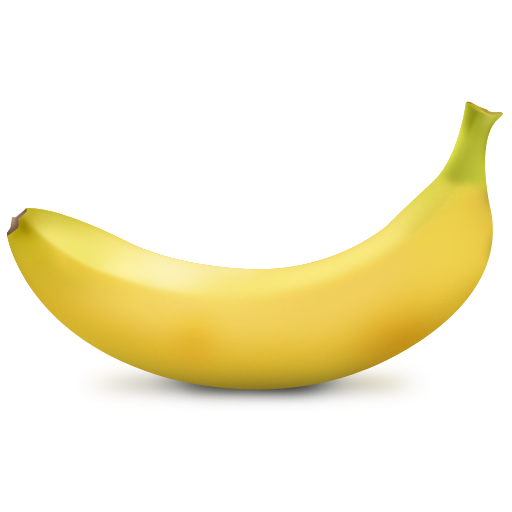
\includegraphics[scale=0.1]{banana.png}

        \subsection{Float: figure environment}
            Figure~\ref{fig:ballon} and figure~\ref{fig:banana} in float environment\\
            \vspace{1cm}\\
            \begin{figure}[htbp]
                \begin{center}
                    
\includegraphics[scale=0.1]{ballon.jpg}
                    \caption{This is a ballon.}
                    \label{fig:ballon}
                    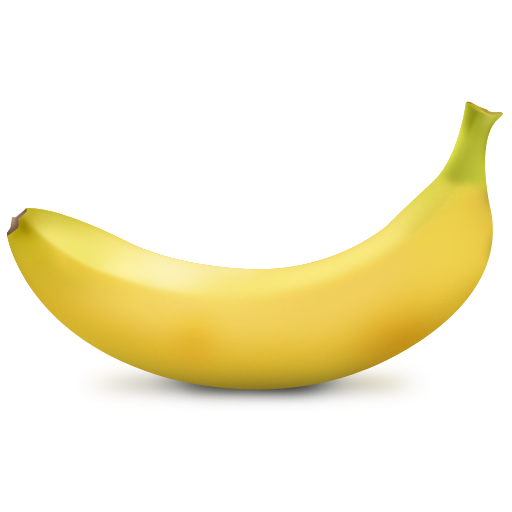
\includegraphics[scale=0.1]{banana.png}
                    \caption{This is a banana.}
                    \label{fig:banana}
                \end{center}
            \end{figure}
    \section{Conclusion}
            Adding immage to an article
\end{document}